\documentclass{article}


\usepackage{arxiv}

\usepackage[utf8]{inputenc} % allow utf-8 input
\usepackage[T1]{fontenc}    % use 8-bit T1 fonts
\usepackage{hyperref}       % hyperlinks
\usepackage{url}            % simple URL typesetting
\usepackage{booktabs}       % professional-quality tables
\usepackage{amsfonts}       % blackboard math symbols
\usepackage{nicefrac}       % compact symbols for 1/2, etc.
\usepackage{microtype}      % microtypography
\usepackage{lipsum}
\usepackage{graphicx}
\usepackage{amsmath,amssymb}
\usepackage{algorithm}
\usepackage{algorithmicx}
\usepackage{algpseudocode}
\graphicspath{ {./images/} }
\usepackage{fixmath}
\usepackage{graphicx}
\usepackage{subcaption}


\DeclareMathOperator{\EX}{\mathbb{E}}% expected value

\title{FREE vs FAST adversarial training}
\author{Giuseppe Capaldi\\
	University of Rome "La Sapienza"\\
	\texttt{capaldi.1699498@studenti.uniroma1.it}\\
	\And Gianluca Capozzi\\
	University of Rome "La Sapienza"\\
	\texttt{capozzi.1693255@studenti.uniroma1.it}\\
}

\begin{document}


\maketitle

\begin{abstract}
In this work we propose a comparison between two methods for adversarial
training: Free and Fast. We started from [Shafahi et al.] \cite{ShafahiEtAl2019b} trying to reach their conclusions, in particular the choice of \textit{m} as a crucial parameter in its algorithm. Then we did the same 
for [Wong et al.] \cite{WongEtAl2020}, with regard to the crucial parameter $\alpha$.
We then chose from our experiments  the best among these two parameters to enforce a comparison between the two methods presented in the above cited papers, comparing validation and robustness accuracies along with required train times. Finally we analyzed and compared Resnet50 and PreActResNet18 results both in Free and Fast adversarial training.\\
 The code is available at
\url{https://github.com/not-a-genius/neuralNetworkExam}.
\end{abstract}

\section{Introduction}
Adversarial training is a method for training robust deep neural networks,
training on adversarial examples as a defense against adversarial attacks. This
is typically considered to be more expensive than standard training due to the
necessity of constructing adversarial examples via a first-order method like
projected gradient descent (PGD). The papers presented show that it is possible
to train empirically robust models using methods no more costly than standard
training in practice. These methods show results comparable to train a model
against PGD but at lower cost in terms of computational time. The goal of
adversarial training is to learn a model which is not only accurate on the data
(accuracy on train and test data) but also accurate on adversarially perturbed
versions of the data (i.e. accuracy on images perturbed using the PGD attack).  
This leads to particular attention at the results we obtained after adversarial
training experiments, aware of the presence of an acceptable compromise in
accuracy, given a large increase in robustness due to the tradeoff between
robustness and generalization \cite{TsiprasEtAl, ZhangEtAl2019a,
ShafahiEtAl2019a}.

\subsection{Related Works}
Our work is based on “Adversarial training for free!” paper
\cite{ShafahiEtAl2019b}, that presented an algorithm able to eliminate the
overhead cost of generating adversarial examples by recycling the gradient
information computed when updating the model parameters. While researching
related work in the field we discovered a more recent paper, called "Fast is
better than free: Revisiting adversarial training" \cite{WongEtAl2020}
presenting an improvement of an already known method called FGSM, previously
considered ineffective due to what the paper calls “catastrophic overfitting”.
This failure condition is preventable with the use of random initialization
points. Moreover the same paper reported a further acceleration in training even
for the Free algorithm, thanks to standard techniques for efficient training,
including cyclic learning rate and mixed-precision arithmetic. This caught our
interest and we decided to try to replicate the reported results and compare
them with our implementation, in order to confirm or deny these thesis.

\subsection{Dataset and architecture}

We decided to choose CIFAR-10 as the dataset on which our experiments have been
conducted. All of them are run on a single NVIDIA RTX 2070-Super GPU.\\
The CIFAR-10 dataset consists of 60000 32x32 colour images in 10 classes, with
6000 images per class. There are 50000 training images and 10000 test images.
The dataset is divided into five training batches and one test batch, each with
10000 images. The test batch contains exactly 1000 randomly-selected images from
each class. The training batches contain the remaining images in random order,
but some training batches may contain more images from one class than another.
Between them, the training batches contain exactly 5000 images from each
class.\\
We conducted adversarial training examples using as models ResNet50 and
PreActResNet18. Both ResNet50 and PreActResnet18 results have been reported and
compared between them, under the same conditions. 


\section{Adversarial Machine Learning}
Adversarial machine learning is a machine learning technique that attempts to
fool models by supplying deceptive input (called also adversarial example).
Adversarial examples exploit the way artificial intelligence algorithms work to
disrupt the behavior of such algorithms. In the past few years, adversarial
machine learning has become an active area of research as the role of AI
continues to grow in many of the applications we use. There’s growing concern
that vulnerabilities in machine learning systems can be exploited for malicious
purposes. The main idea to deal with adversarial examples is represented by
adversarial training; it can be traced back to \cite{GoodfellowEtAl2015}, in
which models were hardened by producing adversarial examples and injecting them
into training data \cite{ShafahiEtAl2019b}.\\
This technique can be summarized as follows: given a network $f_{\theta}$
parametrized by $\theta$, a dataset ($x_i$, $y_i$), a loss function $l$ and a
threat model $\Delta$, the learning problem consists in the following
optimization problem:
\begin{center}
	$min_{\theta}{\sum_{i}l(f_{\theta}(x_i + \delta), y_i)}$
\end{center}
A typical choice for the adversarial model is to take $\Delta = \{\delta :
||\delta||_{\infty} \le \epsilon\}$ for some $\epsilon > 0$.

\section{PGD attack}
The PGD attack is a white-box attack, which means that the attacker has access
to the model's weights, giving to the attacker much more power than a black-box
attack (in which the model's weights are not known), as he can specifically
craft the attack to fool the chosen model without having to rely on transfer
attacks, which often result in human-visible perturbations. The key for
understanding the PGD attack is to frame the research of an adversarial example as a
constrained optimization problem. PGD attempts to find the perturbation that
maximizes the loss of a model on a particular input while keeping the size of
the perturbation smaller than a specified amount referred to as epsilon. This
constraint is usually expressed as the $l_2$ or $l_{\infty}$ norm of the
perturbation and it is added so that the content of the adversarial example is as similar as possible to the unperturbed sample. The PGD algorithm can be summarised with the 4
steps below (although the attacker is free to apply any optimisation
improvements such as momentum, Adam, multiple restarts, etc...):
\begin{enumerate}
	\item Start from a random perturbation in the $l_p$ ball around a sample;
	\item Take a gradient step in the direction of the greatest loss;
	\item Project perturbation back into the $l_p$ ball if necessary;
	\item Repeat steps 2-3 until convergence.
\end{enumerate}
In our case, adversarial training consists simply of putting the PGD attack
inside the training loop, applying a kind of "data augmentation"; in this case,
instead of performing random transformations as a preprocessing step, we create
specific perturbations that best fool the model and indeed adversarially trained
models do exhibit less overfitting when trained on small datasets.\\
The PGD attack is based on the simplest version of what is called Fast Gradient
Sign Method, used to approximate the inner maximization of Delta. This could be
seen as a relatively inaccurate approximation of the inner maximization for
$l_{\infty}$ perturbations, and has the following closed form (as shown in
\cite{GoodfellowEtAl2014}):
\begin{center}
	$\delta^{\star} = \epsilon \cdot sign(\nabla_{x}l(f(x), y))$.
\end{center}
A better approximation of the inner maximization is to take multiple, smaller
FGSM steps of size alpha. When the iteration leaves the threat model, it is
projected back to the set $\Delta$. Multiple restarts within the threat model
$\Delta$ typically improve the approximation of the inner maximization even
further. The combination of all these techniques is the PGD attack. The problem
of such technique is that the number of gradient computations here is
proportional to O(MK) in a single epoch, where M is the size of the dataset and
K is the number of steps taken by the PGD adversary. This is K times greater
than standard training so adversarial training is typically K times slower than
standard training. The pseudo-code of the PGD attack is reported in Algorithm 1.
\begin{algorithm}[H]
	\caption{PGD adversarial training for T epochs, given some radius $\epsilon$,
	adversarial step size $\alpha$ and $K$ PGD steps and a a dataset of size $M$
	for a network $f_{\theta}$}
	\begin{algorithmic}[1]
		\For{$t = 1...T$} \For{$i = 1...M$} \State// Perform PGD adversarial attack
		\State $\delta = 0$ // or randomly initialized \For{$j = 1 ... K$} \State
		$\delta = \delta + \alpha\cdot sign(\nabla_{\delta}l(f_{\delta}(x_i +
		\delta), y_i))$ \State $\delta = max(min(\delta, \epsilon), -\epsilon)$
		\EndFor \State$\theta = \theta - \nabla_{\theta}l(f_{\theta}(x_i + \delta),
		y_i)$ // Update model weights with some optimizer, e.g. SGD \EndFor \EndFor
	\end{algorithmic}
\end{algorithm}
The execution of K-PGD in \cite{MadryEtAl2017} took four days on a Titan X (with
model WideResNet and dataset CIFAR-10). This led us to consider the reported
results \cite{ShafahiEtAl2019b},\cite{WongEtAl2020}, obtained using K-PGD
adversarial training, without running them directly.
\section{DAWNBench improvements}
The top submissions to the DAWNBench competition have shown that CIFAR10 (and
also ImageNet) classifiers can be trained spending significantly less
computational time and at much lower cost than traditional learning methods.
There are two general approaches that have an effective impact on the
convergence rate and computational speed of standard training. They are:
\begin{itemize}

\item \textbf{Cyclic Learning Rate}: used for improving convergence and reducing
the amount of tuning required when training networks. When a cyclic schedule is
used, the number of epochs required for training deep networks is drastically
reduced in particular, in the case of a CIFAR10 classifier, then convergence is
achieved in tens of epochs instead of hundreds.
\item \textbf{Mixed-precision arithmetic}: this improvement can be used only
with newer GPU architectures (which come with tensor cores specifically built
for rapid half-precision calculations). The key idea is that using
mixed-precision arithmetic when training deep networks can also provide
significant speedups for standard training. Moreover, this drastically reduces
memory utilization. Both these techniques are adopted for use in our
experiments, allowing us to drastically reduce the number of training epochs as
well as the runtime on GPU  infrastructure with tensor cores, while using modest
amounts of computational resources. 
\end{itemize}
\section{Free Adversarial training for free!}

Free adversarial training \cite{ShafahiEtAl2019b} claims to reduce the overhead
compared to natural training. The idea behind the improved algorithm is the
computation of ascent step by reusing the backward pass needed for the descent
step. So the gradient with respect to the network parameters is computed on the
backward pass and later on this same backward pass the gradient of the loss with
respect to the input image is also computed.\\
In order to allow multiple adversarial updates on the same image the training is
made on the same minibatch \textit{m} times in a row. Every minibatch is
repeated m times before switching to the next minibatch (“minibatch replays”),
so the number of epochs can be considered as the number of epochs divided by \textit{m},
such that the overall number of training iterations remains constant. Note that
perturbations are not reset between mini-batches. The value of this parameter is
shown to be crucial, since increasing m comes with the risk of increasing
generalization error revealing  the presence of a trade-off: robustness is
increased at the cost of validation accuracy on natural images.\\
The pseudocode of Free is shown in Algorithm 2.

\begin{algorithm}[H]
	\caption{"Free" Adversarial Training (Free-m)}
	\begin{algorithmic}[1]
		\Require Training samples X, perturbation bound $\epsilon$, learning rate
		$\tau$, hop steps $m$ \State Initialize $\theta$ \State $\delta$
		$\leftarrow$ 0 \For{$epoch = 1...N_{ep}/m$} \For{$minibatch \; B \in X$}
		\For{$i = 1...m$} \State // Update $\theta$ with stochastic gradient descent
		\State $g_{\theta} \leftarrow \EX_{(x,y) \in B} \nabla_{\theta} [l(x+\delta,
		y, \theta)]$ \State $g_{adv} \leftarrow \nabla_{x} l(x+\delta, y, \theta)$
		\State $\theta \leftarrow \theta - \tau g_{\theta}$ \State // Use gradients
		calculated for the minimization step to update $\delta$ \State $\delta
		\leftarrow + \epsilon \cdot sign(g_{adv})$ \State $clip(\delta, -\epsilon,
		\epsilon)$ \EndFor \EndFor \EndFor
	\end{algorithmic}
\end{algorithm}
In the choice of m one problem may arise: it's possible that catastrophic
forgetting happens, e.g. when all the “informative” images of one class are in
the first few mini-batches. In this extreme case, we do not see useful examples
for most of the epoch, and forgetting may occur. How much does mini-batch replay
hurt generalization? To answer the question we followed \cite{ShafahiEtAl2019b}
approach trying different values of \textit{m}, reaching the same results: dropoff in
accuracy for small \textit{m}, while we see an inversion in PGD and test
accuracy for high values of it. On CIFAR-10 effective robustness can be reached
with values of $m \leq 10$, our best results have been obtained with $m = 8$.\\
It is known that adversarially trained classifiers, e.g. classifiers trained
against PGD,  have generative
behaviours. When an image is perturbed from one class to another, it adopts
features that make it “look” like its adopted class, to a human eye. Free
trained models exhibit this benefit and also smooth and flattened loss surface.
Indeed, standard adversarially trainined classifiers show the property to have a
flatten and smooth loss landscape while some defenses work by “masking” the
gradients. This techniques makes it difficult to identify adversarial examples
using gradient methods, even though adversarial examples remain present.
Reference \cite{EngstromEtAl2018} argues that gradient masking adds little
security, free training does not operate by masking gradients and uses a rough
loss surface.

\subsection{Experiments results}
In this section, we present the results of our experiments conducted using Free
method and varying the number of minibatch replays. We can notice that the train
time increase as \textit{m} increases as expected but in the case of $m=10$ we
got values of accuracies lower than $m=8$.\\
All experiments using Free adversarial training in this section are carried out
with the same number of epochs and epsilon value $\epsilon = 8/255$. We are
interested in evaluating the accuracy of the model against the natural images and
the accuracy against images perturbed using the PGD attack. In particular, we
ran PGD using three different values for the number \textit{K} of iterations,
which are \{10, 20, 50\}. The number of random restarts used for PGD is 1; all the
other hyper-parameters are the same used by [Shafahi et al.] in
\cite{ShafahiEtAl2019b}. The implementation of Free provided by [Wong et al.] in
\cite{WongEtAl2020} includes also the optimization of cyclic learning rate and
mixed-precision.\\
The following table shows the results when the used model is PreactResNet18:
\begin{table}[hbt!]
\begin{tabular}{|c|l|l|l|l|l|l|p{2cm}|}
\hline
\multicolumn{1}{|l|}{{ }}        & \multicolumn{4}{c|}{{ \textbf{Accuracy using
PreActResNet18}}}
& \multicolumn{3}{l|}{{ }}
\\ \hline
{ \textbf{Minibatch-replay (m)}} & \multicolumn{1}{p{1.5cm}|}{{ \textbf{Natural
Images}}} & \multicolumn{1}{c|}{{ \textbf{PGD-10}}} & \multicolumn{1}{c|}{{
\textbf{PGD-20}}} & \multicolumn{1}{c|}{{ \textbf{PGD-50}}} &
\multicolumn{1}{c|}{{ \textbf{Epoch}}} & \multicolumn{1}{p{1.5cm}|}{{
\textbf{Train Time (min)}}} & \multicolumn{1}{p{1.5cm}|}{{ \textbf{Avg Epoch
Time (sec)}}} \\ \hline
{ \textit{m} = 2}                & { 0.895}
& { 0.324}                                & { 0.297}
& { 0.290}                                & { 45}
& { 22 }                               & { 29.4 }
\\ \hline
{ \textit{m} = 4}                & { 0.867}
& { 0.471}                                & { 0.457}
& { 0.451}                                & { 45}
& { 44 }                               & { 58.2 }
\\ \hline
{ \textit{m} = 8}                & { 0.839}
& { 0.498}                                & { 0.486}
& { 0.483}                                & { 45}
& { 88 }                               & { 117 }
\\ \hline
{ \textit{m} = 10}               & { 0.821}
& { 0.490}                                & { 0.482}
& { 0.479}                                & { 45}
& { 108 }                              & { 143.4 }
\\ \hline
\end{tabular}
\end{table}

\newpage

\begin{figure}[hbt!]
  \centering
  \begin{subfigure}[b]{0.4\linewidth}
    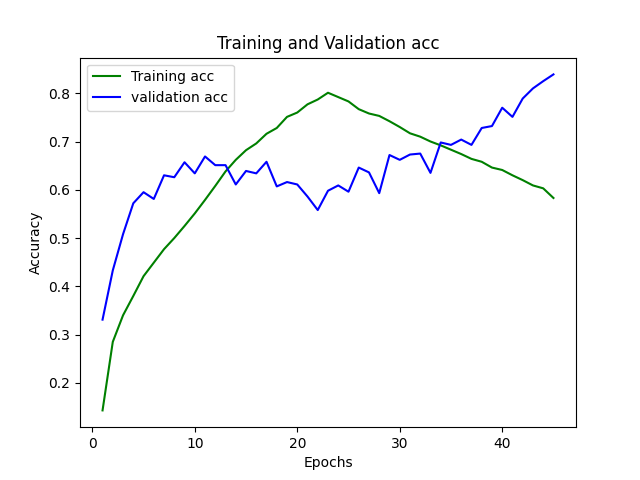
\includegraphics[width=\linewidth]{images/FreePre/free2.png}
    \caption{ Train and validation accuracies results.}
  \end{subfigure}
  \begin{subfigure}[b]{0.4\linewidth}
    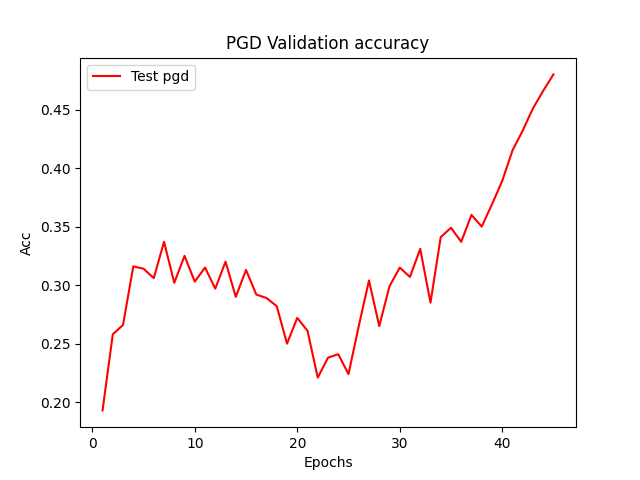
\includegraphics[width=\linewidth]{images/FreePre/free5.png}
    \caption{PGD validation accuracy}
  \end{subfigure}
  \caption{Free Adversarial training using PreActResnet18 (epsilon = 8/255, \textit{m} = 8, batch size = 128,  epochs = 45)}
  \label{fig:coffee}
\end{figure}

The following results are related to the training and evaluation based on
ResNet50 model instead of PreActResnet18. The number of epochs has been
increased to 90 to see the impact on the accuracy in the long run. 


%Figure \ref{fig:boat1} shows a test and validation accuracy.


\begin{table}[hbt!]
\centering
\begin{tabular}{|c|c|l|l|l|l|l|}
\hline
\multicolumn{1}{|l|}{}        & \multicolumn{2}{c|}{\textbf{Accuracy using
ResNet50}}                               & \multicolumn{3}{l|}{\textbf{}}
& \textbf{}                                \\ \hline
\textbf{Minibatch-replay (m)} & \textbf{Natural Images}                      &
\multicolumn{1}{c|}{\textbf{PGD-50}} & \multicolumn{1}{c|}{\textbf{Epoch}} &
\multicolumn{1}{p{1.5cm}|}{\textbf{Train Time (min)}} &
\multicolumn{1}{p{1.5cm}|}{\textbf{Avg Epoch Time (sec)}} &
\multicolumn{1}{c|}{\textbf{Batch size}} \\ \hline
\textit{m} = 8       & \multicolumn{1}{l|}{0.735} & { 0.404}         & { 90}           &
{ 118}                     & { 78.6}                        & { 128}
\\ \hline
\end{tabular}
\end{table}


\begin{figure}[hbt!]
  \centering
  \begin{subfigure}[b]{0.4\linewidth}
    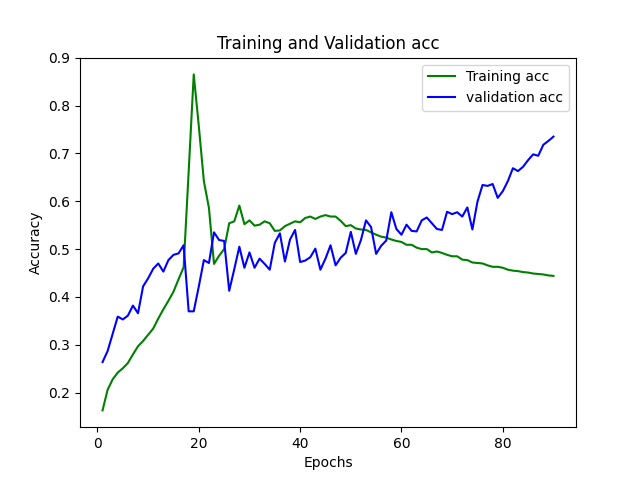
\includegraphics[width=\linewidth]{images/FreeResnet/Figure_2.png}
    \caption{ Train and validation accuracies results.}
  \end{subfigure}
  \begin{subfigure}[b]{0.4\linewidth}
    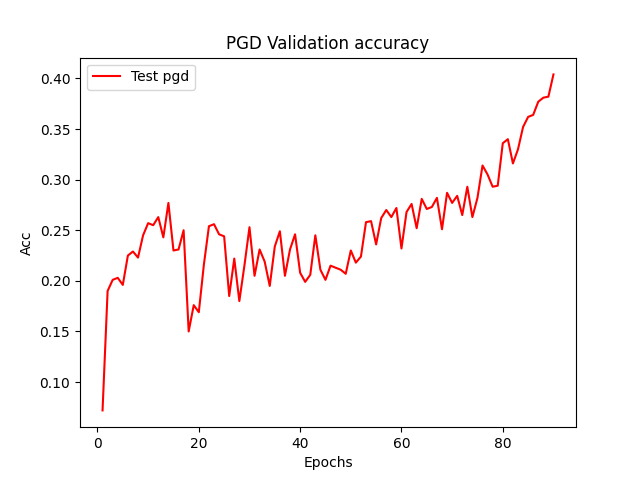
\includegraphics[width=\linewidth]{images/FreeResnet/Figure_5.png}
    \caption{PGD validation accuracy}
  \end{subfigure}
  \caption{Free Adversarial training using ResNet50 (epsilon = 8/255, \textit{m} = 8, batch size = 128,  epochs = 90)}
  \label{fig:coffee}
\end{figure}


\section{Fast is better than free}

[Wong et al.] in \cite{WongEtAl2020} consider it possible to have shorter
adversarial training times than the Free method proposed by [Shafahi et al.] in
\cite{ShafahiEtAl2019b} using a modified version of the simple FGSM method,
called Fast; if we compare the data from the two original papers [Shafahi et
al.] in \cite{ShafahiEtAl2019b} and [Wong et al.] in \cite{WongEtAl2020}, we can see
that the Free method requires 785 minutes for achieving a good robustness on
CIFAR-10 against PGD while the Fast method, in order to achieve the same
robustness, requires 12.17 minutes. Similar results about the speed-up in
adversarial training time can been observed if the chosen dataset is Imagenet.\\
A key difference between Fast/FGSM and Free adversarial training, is that in the
latter the perturbation from the previous minibatch is a reasonable starting
point for the next minibatch, while FGSM can be used as it is, just starting
from a non-zero initial perturbation.\\
So, “Fast” adversarial training is just standard FGSM with random non-zero
initialization for the perturbation and this is claimed to be as effective as
PGD adversarial training. This idea of non-zero random initial perturbation was
already introduced by [Tramèr et al.] in \cite{TramerEtAl2017} but, the key
difference between this implementation and Fast is that, the first one uses a
more restricted random initialization and step size, which doesn't give a robust
model against PGD attack.  So, for this adversarial training, one crucial
parameter is the step size $\alpha$ that shows results on par with “Free” ones
only choosing values in a particular interval. Indeed, two failure modes arise:
\begin{itemize}

\item a step size too small ($\alpha$ =$\epsilon$) would mean a zero-initialized
perturbation and lead to a too weak defense
\item a step size too large ($\alpha$ = $2\epsilon$) will lead to a model
overfitted, restricted to specific threats (“catastrophic overfitting”).
\end{itemize}

A good compromise for these parameters is shown to be: $\alpha$ = 1.25,
$\epsilon$ = 10/255.\\
Another key difference is that FGSM does not need to repeat mini-batches, but
needs two backward passes to compute gradients separately from the perturbation
and the model weights. From a computational complexity point of view this means
that an epoch of FGSM is equivalent to two epochs of standard training.

\begin{algorithm}[H]
	\caption{FGSM adversarial training for T epochs}
	\begin{algorithmic}[1]
		\Require Dataset of size M, radius $\epsilon$, K PGS steps, step size
		$\alpha$ \For{$t = 1...T$} \For{$i = 1...M$} \State // Perform FGSM
		adversarial attack \State $\delta = Uniform(-\epsilon, \epsilon)$ \State
		$\delta = \delta + \alpha \cdot sign(\nabla_{\delta} l(f_{\theta}(x_i +
		\delta), y_i))$ \State $\delta = max(min(\delta, \epsilon), -\epsilon)$
		\State // Update model weights with some optimizer, e.g. SGD \State $\theta
		= \theta - \nabla_{\theta} l(f_{\theta}(x_i + \delta), y_i)$ \EndFor \EndFor
	\end{algorithmic}
\end{algorithm}

\subsection{Experiments results}

All experiments using FGSM adversarial training in this section are carried out
with the same number of epochs, epsilon value $\epsilon = 8/255$. We ran PGD using three different values for the number \textit{K} of iterations,
which are \{10, 20, 50\}. The number of random restarts used for PGD is 1
while the remaining hyperparameters are those used by [Wong et al.]
in \cite{WongEtAl2020}. Speedup is determined also by the optimization of cyclic learning rate and
mixed-precision.\\
The following results are related to the training and evaluation based on PreActResnet18 model. 
\begin{center}
\begin{table}[hbt!]
\begin{tabular}{|c|l|l|l|l|l|l|l|l|}
\hline
\multicolumn{1}{|l|}{{ }} & \multicolumn{4}{c|}{{ \textbf{Accuracy using
PreActResNet18}}}
& \multicolumn{4}{l|}{{ }}
\\ \hline
{ \textbf{Step-size}}     & \multicolumn{1}{p{1.5cm}|}{{ \textbf{Natural
Images}}} & \multicolumn{1}{c|}{{ \textbf{PGD-10}}} & \multicolumn{1}{c|}{{
\textbf{PGD-20}}} & \multicolumn{1}{c|}{{ \textbf{PGD-50}}} &
\multicolumn{1}{c|}{{ \textbf{Epoch}}} & \multicolumn{1}{p{1.5cm}|}{{
\textbf{Train Time (min)}}} & \multicolumn{1}{p{1.5cm}|}{{ \textbf{Avg Epoch
Time (sec)}}} & \multicolumn{1}{c|}{{ \textbf{Batch size}}} \\ \hline
{ $\alpha = 10$}       & { 0.847}                                        & {
0.480}                                & { 0.463}
& { 0.450}                                & { 45}
& { 21 }                               & { 28.8 }
& { 128}                                      \\ \hline
{ $\alpha = 10$}       & { 0.850}                                        & {
0.454}                                & { 0.438}
& { 0.434}                                & { 45}
& { 20 }                               & { 25.8 }
& { 256}                                      \\ \hline
{ $\alpha = 16$}       & { 0.856}                                        & { 0}
& { 0}                                    & { 0}
& { 45}                                  & { 21 }
& { 28.2 }                                 & { 128}
\\ \hline
{ $\alpha = 16$}       & { 0.87}                                         & { 0}
& { 0}                                    & { 0}
& { 45}                                  & { 20 }
& { 26.4 }                                 & { 256}
\\ \hline
\end{tabular}
\end{table}
\end{center}


\begin{figure}[hbt!]
  \centering
  \begin{subfigure}[b]{0.4\linewidth}
    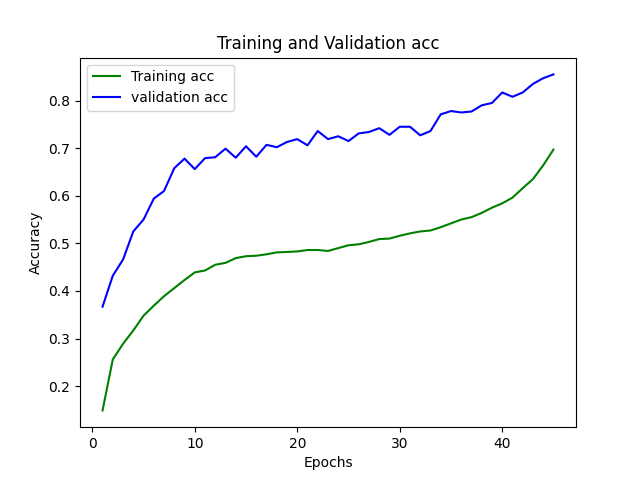
\includegraphics[width=\linewidth]{images/FastPre/fast2.png}
    \caption{ Train and validation accuracies results.}
  \end{subfigure}
  \begin{subfigure}[b]{0.4\linewidth}
    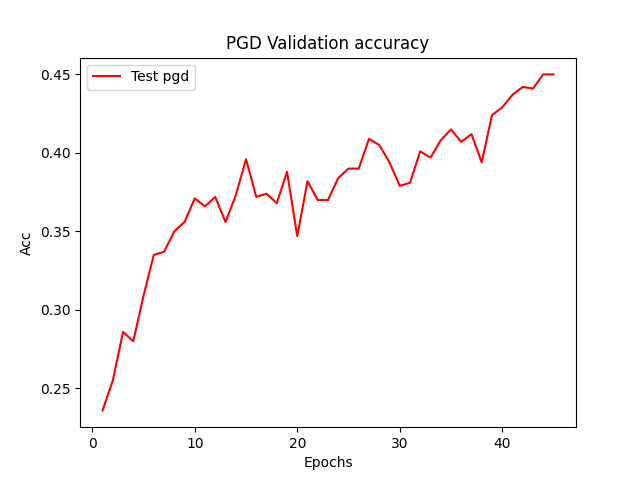
\includegraphics[width=\linewidth]{images/FastPre/fast5.png}
    \caption{PGD validation accuracy}
  \end{subfigure}
  \caption{FGSM Adversarial training using PreActResNet18 (epsilon = 8/255, \textit{m} = 8, batch size = 128, epochs = 45)}
  \label{fig:coffee}
\end{figure}

\newpage

The following results are related to the training and evaluation based on
ResNet50 model instead of PreActResnet18. The number of epochs has been
increased to 90 to see the impact on the accuracy in the long run. 

\begin{table}[hbt!]
\begin{tabular}{|c|c|l|l|l|l|l|}
\hline
\multicolumn{1}{|l|}{}    & \multicolumn{2}{c|}{\textbf{Accuracy using
Resnet50}}                               & \multicolumn{4}{l|}{\textbf{}}
\\ \hline
\textbf{Step-size}        & \textbf{Natural Images}                      &
\multicolumn{1}{c|}{\textbf{PGD-50}} & \multicolumn{1}{c|}{\textbf{Epoch}} &
\multicolumn{1}{c|}{\textbf{Train Time (min)}} & \multicolumn{1}{c|}{\textbf{Avg
Epoch Time (sec)}} & \multicolumn{1}{c|}{\textbf{Batch size}} \\ \hline
$\alpha$ = 10/255 & \multicolumn{1}{l|}{0.766} & { 0.391}         & { 90}
& { 28.18}                   & { 18.78}                       & { 128}
\\ \hline
\end{tabular}
\end{table}


\begin{figure}[hbt!]
  \centering
  \begin{subfigure}[b]{0.4\linewidth}
    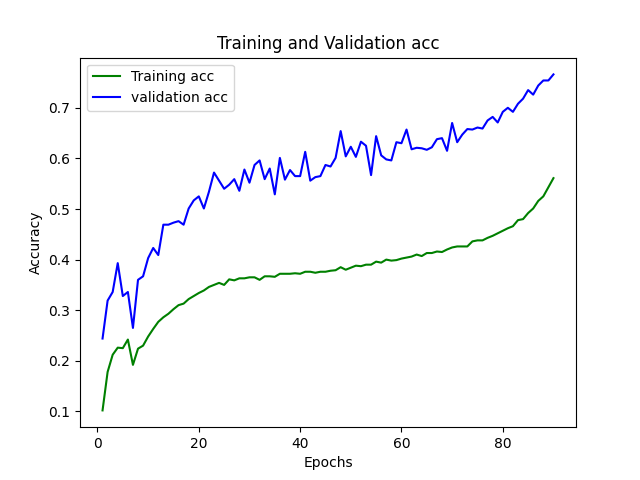
\includegraphics[width=\linewidth]{images/FastResnet/Figure_2.png}
    \caption{ Train and validation accuracies results.}
  \end{subfigure}
  \begin{subfigure}[b]{0.4\linewidth}
    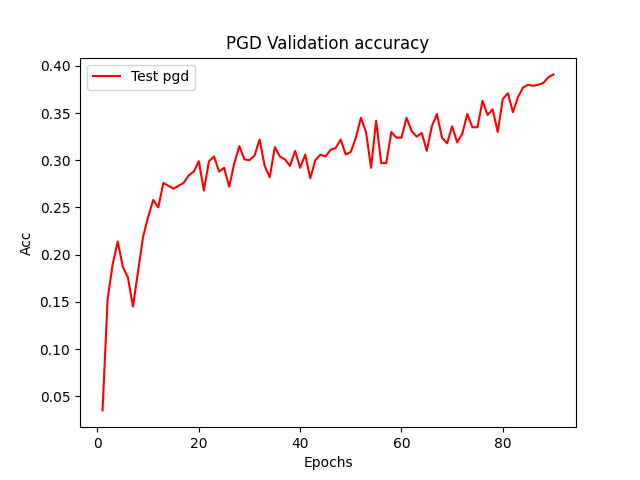
\includegraphics[width=\linewidth]{images/FastResnet/Figure_5.png}
    \caption{PGD validation accuracy}
  \end{subfigure}
  \caption{FGSM Adversarial training using Resnet50 (epsilon = 8/255, \textit{m} = 8, batch size = 128, epochs = 90)}
  \label{fig:coffee}
\end{figure}
\newpage


\section{Final Experiments}
In order to ease the training and the experiments using different parameters we also developed a single python script that load user preferences (hyperparameters and general parameters) from an editable config file. In "configs.ini" file the user can choose among three different modalities (sequential running of free adv. training and then fgsm, only free adv. training or only fast) and change hyperparameters  (batch size, epsilon, etc...) along with common parameters (name of the model, output filename, etc...).

\subsection{Free vs Fast using PreActResnet18}
In this section we compare the best results we obtained from the precedent
experiments, then showing the evolution of validation accuracy in these two
methods using Resnet50 as model. \\
The following table contains the best \textit{m} and batch size values for free method,
obtained from the different free experiments compared with the best step size
and batch size for FGSM. 
\begin{table}[hbt!]
\begin{tabular}{|l|p{2.1cm}|c|l|l|l|l|l|}
\hline
              & \multicolumn{1}{l|}{}         &
              \multicolumn{2}{c|}{\textbf{Accuracy using PreactResnet18}}
              & \multicolumn{3}{l|}{\textbf{}}
              & \textbf{}                                \\ \hline
 & \textbf{Minibatch-replays (m) / step size ($\alpha$)} & \textbf{Natural
 Images}                      & \multicolumn{1}{c|}{\textbf{PGD-50}} &
 \multicolumn{1}{c|}{\textbf{Epoch}} & \multicolumn{1}{p{1cm}|}{\textbf{Train
 Time (min)}} & \multicolumn{1}{p{1cm}|}{\textbf{Avg Epoch Time (sec)}} &
 \multicolumn{1}{c|}{\textbf{Batch size}} \\ \hline
\textbf{FREE} & \textit{m} = 8 & \multicolumn{1}{l|}{0.845} & { 0.485}         & { 90}
& { 176}                     & { 117}                         & { 128}
\\ \hline
\textbf{FAST} & $\alpha = 10/255$       & \multicolumn{1}{l|}{0.836} & { 0.434}
& { 90}           & { 43}                     & { 28}                         &
{ 128}               \\ \hline
\end{tabular}
\end{table}

\begin{figure}[hbt!]
  \centering
  \begin{subfigure}[b]{0.4\linewidth}
    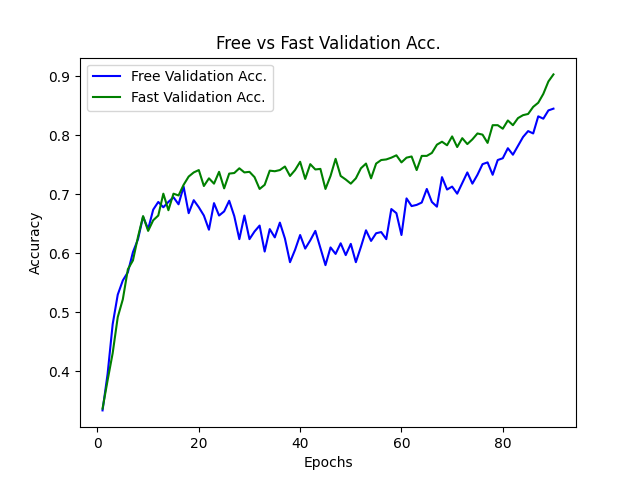
\includegraphics[width=\linewidth]{images/preComp/Figure_1.png}
    \caption{ Free vs Fast, Validation accuracies.}
  \end{subfigure}
  \begin{subfigure}[b]{0.4\linewidth}
    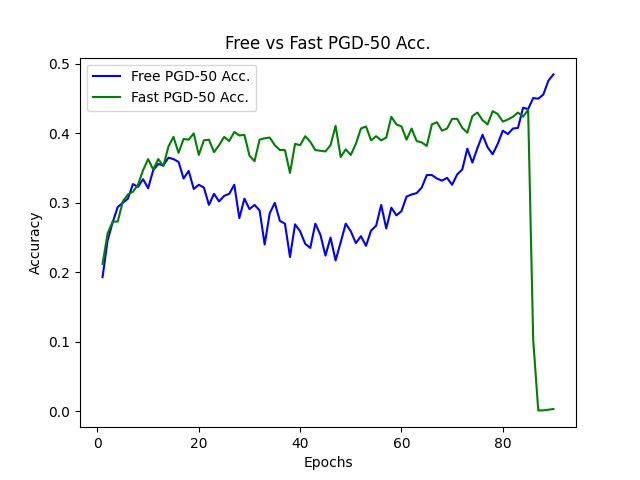
\includegraphics[width=\linewidth]{images/preComp/Figure_2.png}
    \caption{Free vs Fast, PGD validation accuracies.}
  \end{subfigure}
  \caption{Comparing results for Adversarial training using PreActResNet18 in Free vs Fast.}
  \label{fig:coffee}
\end{figure}

\subsection{Free vs Fast using ResNet50}
In this section we compare the best results we obtained from the precedent
experiments, then showing the evolution of validation accuracy in these two
methods when using Resnet50 as model. \\
The following table contains the best \textit{m} and batch size values for free method,
obtained from the different free experiments compared with the best step size
and batch size for FGSM. 

\begin{table}[hbt!]
\begin{tabular}{|l|p{2.1cm}|c|l|l|l|l|l|}
\hline
              & \multicolumn{1}{l|}{}         &
              \multicolumn{2}{c|}{\textbf{Accuracy using ResNet50}}
              & \multicolumn{3}{l|}{\textbf{}}
              & \textbf{}                                \\ \hline
 & \textbf{Minibatch-replays (m) / step size ($\alpha$)} & \textbf{Natural
 Images}                      & \multicolumn{1}{c|}{\textbf{PGD-50}} &
 \multicolumn{1}{c|}{\textbf{Epoch}} & \multicolumn{1}{p{1cm}|}{\textbf{Train
 Time (min)}} & \multicolumn{1}{p{1cm}|}{\textbf{Avg Epoch Time (sec)}} &
 \multicolumn{1}{c|}{\textbf{Batch size}} \\ \hline
\textbf{FREE} & \textit{m} = 8 & \multicolumn{1}{l|}{0.735} & { 0.404}         & { 90}
& { 118}                     & { 79}                         & { 128}
\\ \hline
\textbf{FAST} & $\alpha = 10/255$       & \multicolumn{1}{l|}{0.766} & { 0.391}
& { 90}           & { 29}                     & { 19}                         &
{ 128}               \\ \hline
\end{tabular}
\end{table}

\newpage


\begin{figure}[hbt!]
  \centering
  \begin{subfigure}[b]{0.4\linewidth}
    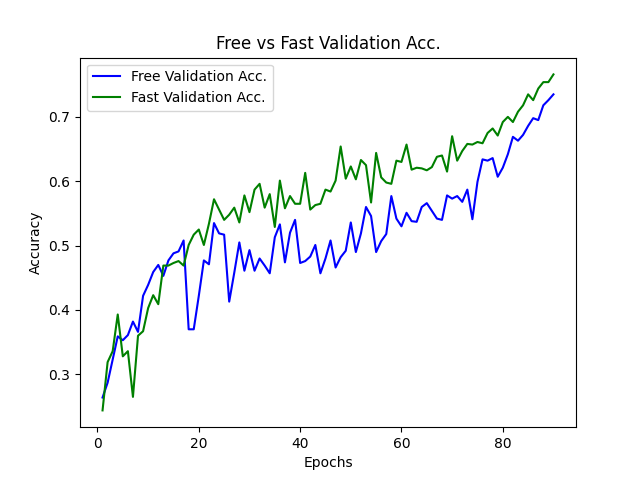
\includegraphics[width=\linewidth]{images/resComp/Figure_1.png}
    \caption{ Free vs Fast, Validation accuracies.}
  \end{subfigure}
  \begin{subfigure}[b]{0.4\linewidth}
    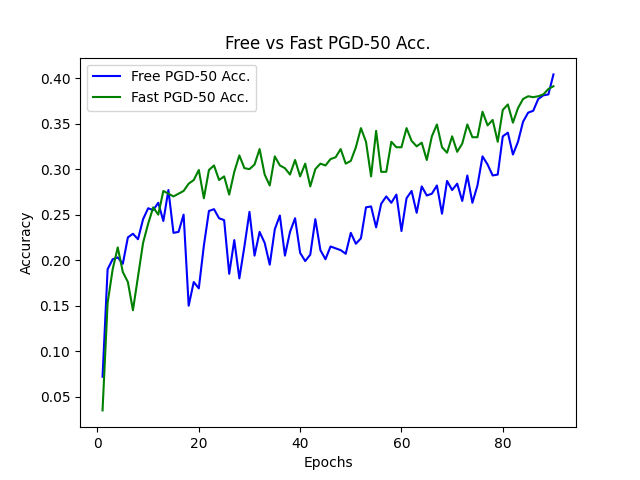
\includegraphics[width=\linewidth]{images/resComp/Figure_2.png}
    \caption{Free vs Fast, PGD validation accuracies.}
  \end{subfigure}
  \caption{Comparing results for Adversarial training using Resnet50 in Free vs Fast.}
  \label{fig:coffee}
\end{figure}

\subsection{PreAct18 vs ResNet50}
In the following two charts we compare the evolution of Free adv. learning using
the two different models ResNet50 and PreActResnet18. 



\begin{figure}[hbt!]
  \centering
  \begin{subfigure}[b]{0.4\linewidth}
    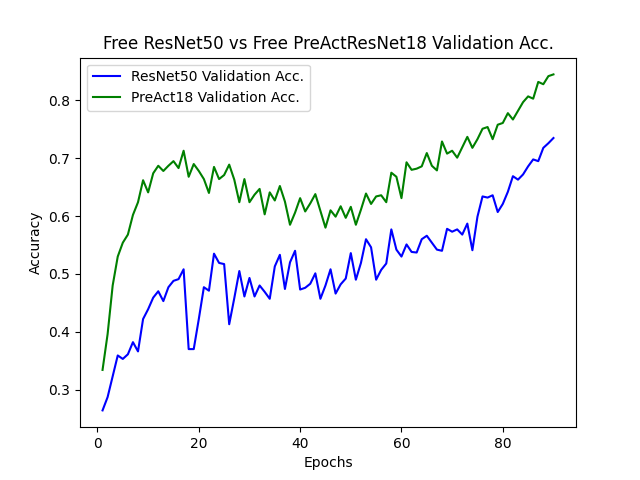
\includegraphics[width=\linewidth]{images/freeComp/Figure_1.png}
    \caption{Preact18 vs Resnet50  Validation accuracies.}
  \end{subfigure}
  \begin{subfigure}[b]{0.4\linewidth}
    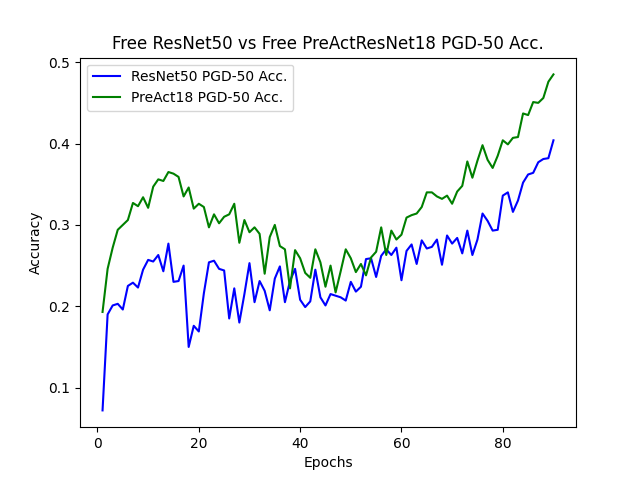
\includegraphics[width=\linewidth]{images/freeComp/Figure_2.png}
    \caption{Preact18 vs Resnet50 PGD validation accuracies.}
  \end{subfigure}
  \caption{Free Adversarial training (epsilon = 8/255, \textit{m} = 8, batch size = 128,  epochs = 90)}
  \label{fig:coffee}
\end{figure}


\begin{figure}[hbt!]
  \centering
  \begin{subfigure}[b]{0.4\linewidth}
    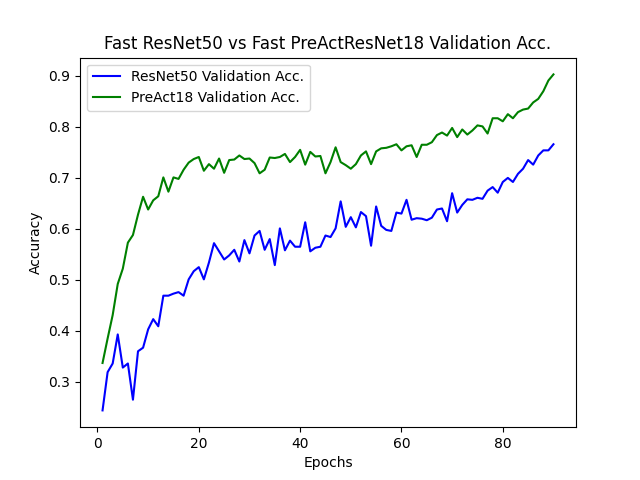
\includegraphics[width=\linewidth]{images/fastComp/Figure_1.png}
    \caption{ Preact18 vs Resnet50 Validation accuracies.}
  \end{subfigure}
  \begin{subfigure}[b]{0.4\linewidth}
    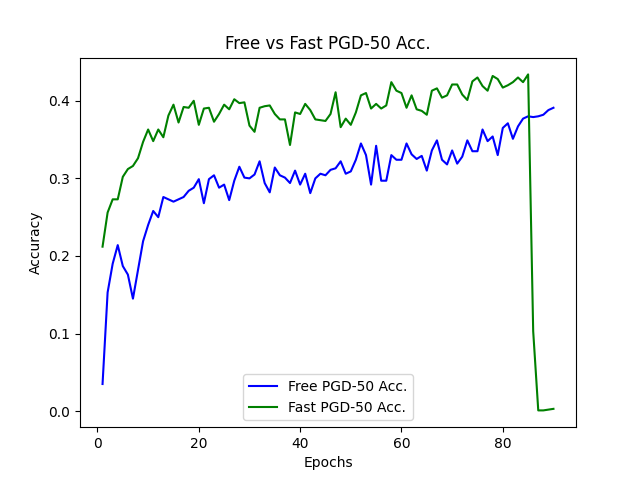
\includegraphics[width=\linewidth]{images/fastComp/Figure_2.png}
    \caption{Preact18 vs Resnet50 PGD validation accuracies.}
  \end{subfigure}
  \caption{Fast Adversarial training (epsilon = 8/255, $\alpha$ = 10/255, batch size = 128,  epochs = 90)}
  \label{fig:coffee}
\end{figure}



\newpage
\section{Conclusions}
Our experiments confirm minibatch-replays (\textit{m}) as a crucial parameter regarding free method, that needs to be tuned trying to reach a trade-off between test and robustness accuracies.\\
In Fast instead step size ($\alpha$) value is a crucial parameter, highly impactful on robust accuracy. We reached a “catastrophic overfitting” obtaining a null PGD accuracy value passing from a step size of value 10/255 to a step size of value 16/255. 
[Wong et al.]'s paper \cite{WongEtAl2020} was useful to reconsider FGSM as a
feasible method for adversarial training once step size parameter is tuned
correctly, and how simple optimization operations on learning rate adaptation
(Cyclic Learning Rate) or based on hardware compatibility with mixed precision
computation (Mixed-precision arithmetic) can decrease computation time, with
small efforts. FGSM shows results similar to the ones obtained from the "Free"
method, considering the same number of epochs, but the total training time
suggests FGSM as a faster and better method to speed up adversarial training
compared to free, moreover PreActResnet18 showed better results than Resnet50 for all the considered epochs, based on our experiments on CIFAR-10.   






\begin{thebibliography}{100} 
	\bibitem{TsiprasEtAl} {Dimitris Tsipras, Shibani Santurkar, Logan Engstrom, Alexander Turner, and Aleksander Madry. Robustness may be at odds with accuracy. ICLR, 1050:11, 2018}

	\bibitem{ZhangEtAl2019a} {Hongyang Zhang, Yaodong Yu, Jiantao Jiao, Eric P Xing, Laurent El Ghaoui, and Michael I Jordan. Theoretically principled trade-off between robustness and accuracy. ICML, 2019a.}
	\bibitem{ShafahiEtAl2019a} {Ali Shafahi, W Ronny Huang, Christoph Studer, Soheil Feizi, and Tom Goldstein. Are adversarial examples inevitable? ICLR, 2019a.}
	
	\bibitem{ShafahiEtAl2019b} {Ali Shafahi, Mahyar Najibi, Amin Ghiasi, Zheng Xu,
		John Dickerson, Christoph Studer, Larry S Davis, Gavin Taylor, and Tom
		Goldstein. Adversarial training for free! arXiv preprint arXiv:1904.12843,
		2019b.}
	
	\bibitem{WongEtAl2020} {Eric Wong and Leslie Rice and J. Zico Kolter. Fast is better than free: revisiting adversarial learning, arxiv:2001.03994, 2020.}
	
	\bibitem{GoodfellowEtAl2015} {Ian J Goodfellow, Jonathon Shlens, and Christian Szegedy. Explaining and harnessing adversarial examples. ICLR, 2015.}
	
	\bibitem{GoodfellowEtAl2014} {Ian J Goodfellow, Jonathon Shlens, and Christian Szegedy. Explaining and harnessing adversarial examples. arXiv preprint arXiv:1412.6572, 2014.}
	
	\bibitem{MadryEtAl2017} {Aleksander Madry, Aleksandar Makelov, Ludwig Schmidt, Dimitris Tsipras, and Adrian Vladu. Towards deep learning models resistant to adversarial attacks. ICLR, 2017.}
	
	\bibitem{EngstromEtAl2018} {Logan Engstrom, Andrew Ilyas, and Anish Athalye. Evaluating and understanding the robustness of adversarial logit pairing. arXiv preprint arXiv:1807.10272, 2018.}
		\bibitem{TramerEtAl2017} {Florian Tramèr, Alexey Kurakin, Nicolas Papernot,
		Ian Goodfellow, Dan Boneh, and Patrick Mc- Daniel. Ensemble adversarial
		training: Attacks and defenses. arXiv preprint arXiv:1705.07204, 2017.}
	
\end{thebibliography}
	
\end{document}
